\documentclass[10pt]{article}
\usepackage[utf8]{inputenc}

% General-use Packages
\usepackage{amsmath}
\usepackage{amssymb}
\usepackage{graphicx}
\usepackage[margin=1truein]{geometry}
\usepackage{xcolor}
\usepackage{tikz}
\usepackage{pgfplots}
\usepackage{enumerate}
\usepackage{tcolorbox}

%Document-specific Packages%

\usepackage{sectsty}
\usepackage{scrextend}
\usepackage{mathtools}
\usepackage{etoolbox} % used for the \isempty command
\usepackage{xifthen} % used for \ifthenelse

% Meta
\title{MAT137 Test 3 Notebook}
\author{Ian Huang}
\date{\today}

% Number set macros
\def\Z{{\mathbb Z}}
\def\Q{{\mathbb Q}}
\def\R{{\mathbb R}}
\def\C{{\mathbb C}}
\def\N{{\mathbb N}}

% For graphing
\pgfplotsset{soldot/.style={only marks,mark=*},
             holdot/.style={fill=white,only marks,mark=*},
             compat=1.12}
\usepgfplotslibrary{fillbetween}

% Theorem and Definition boxes
\definecolor{_orange}{HTML}{ff9e54}
\definecolor{_orange2}{HTML}{fff5ed}
\definecolor{_blue}{HTML}{519aed}
\definecolor{_blue2}{HTML}{e8f3ff}
\definecolor{_grey}{HTML}{3b3b3b}

\newenvironment{definition}[1][]{\begin{tcolorbox}[colframe=_orange,colback=_orange2,title=Definition. \ifthenelse{\isempty{#1}}{}{(#1)}
]}{\end{tcolorbox}}
\newenvironment{theorem}[1][]{\begin{tcolorbox}[colframe=_blue,colback=_blue2,title=Theorem. \ifthenelse{\isempty{#1}}{}{(#1)}
]}{\end{tcolorbox}}

% "Solution" box
\newenvironment{solution}{\begin{tcolorbox}[colframe=_grey,colback=white,arc=0pt,outer arc=0pt]}{\end{tcolorbox}}

% Colored "TRUE" and "FALSE" elements
\newcommand{\true}{\textbf{\textcolor[HTML]{26de57}{TRUE}}}
\newcommand{\false}{\textbf{\textcolor[HTML]{f54242}{FALSE}}}

% Definitions for ceiling and floor symbols
\DeclarePairedDelimiter\ceil{\lceil}{\rceil}
\DeclarePairedDelimiter\floor{\lfloor}{\rfloor}

% Definitions for norm symbols
\newcommand\norm[1]{\left\lVert#1\right\rVert}

% Definitions for definite integral evaluations
\newcommand*\eval[3]{\left.#1\right\rvert_{#2}^{#3}}

% Utility Macros
\newcommand{\hr}{\par\noindent\makebox[\linewidth]{\rule{\textwidth}{0.4pt}}\par\vspace{0.1in}}
\newcommand{\emptyline}[0]{\\\hfill$~$\\}
\newenvironment{proof}{\par\textit{\textbf{Proof.}}}{\hfill$\blacksquare$}
\newcommand{\suchthat}{~~\text{s.t.}~~}

% Formatting settings
\sectionfont{\LARGE}
\subsectionfont{\Large}
\subsubsectionfont{\large}
\paragraphfont{\large}

% Disable paragraph indents
\setlength{\parindent}{0pt}

% Configure section numbering
\setcounter{secnumdepth}{2}

% New Page after Section
\AddToHook{cmd/section/before}{\clearpage}

\begin{document}

\maketitle
\vfill

The source code for this notebook as well as others can be found on GitHub
\begin{center}
    \texttt{https://github.com/iahuang/uoft-notebooks}
\end{center}
\tableofcontents
\newpage
\section{Unit 6: Applications of Limits and Derivatives}
\subsection{Related Rates}

\section{Unit 7: The Definition of Integral}
\subsection{Sigma Notation}
The notation for sums uses the capital Greek letter $\Sigma$
$$
    \sum_{i=1}^n a_i=a_1+a_2+\dots+a_n
$$
From a programming perspective, the above statement is equivalent to the following code:
\begin{verbatim}
    sum = 0;
    
    for (n=1; n<=i; n++) {
        sum += a[i];
    }
\end{verbatim}
\subsubsection{Useful Formulas}

\begin{alignat*}{3}
     & \sum_{i=1}^n i   &  & =\frac{n(n+1)}{2}      &  & =1+2+\dots+n       \\
     & \sum_{i=1}^n i^2 &  & =\frac{n(n+1)(2n+1)}{6} &  & =1^2+2^2+\dots+n^2 \\
     & \sum_{i=1}^n i^3 &  & =\frac{n^2(n+1)^2}{4}  &  & =1^3+2^3+\dots+n^3
\end{alignat*}
\subsubsection{Properties}
Let $i_0,n\in\Z$. \emptyline
\textbf{Distributive Property}
$$
    \sum_{i=i_0}^n(c\cdot a_i)=c\left(\sum_{i=i_0}^n a_i\right)
$$
\textbf{Associative/Commutative Property}
$$
    \sum_{i=i_0}^n(a_i+b_i)=\sum_{i=i_0}^na_i+\sum_{i=i_0}^nb_i
$$
\subsection{Supremum and Infimum}
\subsubsection{Definitions}
\begin{definition}
    Let $A\subseteq\R$. Let $c\in\R$.
    \begin{enumerate}
        \item $c$ is an \textbf{upper bound} of $A$ when
              $$\forall x\in A,~x\leq c$$
        \item $c$ is the \textbf{least upper bound} or \textbf{supremum} of $A$ when
              \begin{enumerate}
                  \item $c$ is an upper bound of $A$
                  \item If $b\in\R$ is an upper bound of $A$, then $c\leq b$. In other words,
                        $$
                            \forall b\in\R, x\in A,~x\leq b\implies c\leq b
                        $$
              \end{enumerate}
              We denote this value ``$\sup A$''.
        \item If $\sup A\in A$, then $\sup A=\max A$.
        \item $A$ is \textbf{bounded above} when $A$ has at least one upper bound.
    \end{enumerate}
\end{definition}
This definition can be extended to the definition of infimum. $c$ is a \textit{lower bound} of $A$ when $\forall x\in A,~x\geq c$; $c$ is the \textit{infimum} of $A$ when it is the \textit{greatest upper bound} and so on.
\begin{definition}[Supremum of a Function]
    The \textbf{supremum of a function $f$ on a domain $I$}, denoted {\small$\displaystyle\sup_{x\in I}f(x)$}, is equal to
    $$
        \sup\{f(x):x\in I\}
    $$
\end{definition}
\subsubsection{Theorems}
\begin{theorem}[Lowest Upper Bound Principle]
    Let $A\subseteq\R$. \\
    IF
    \begin{enumerate}
        \item $A$ is bounded above
        \item $A$ is not empty
    \end{enumerate}
    THEN $A$ has a least upper bound.
\end{theorem}
\begin{theorem}
    Let $f$ be a function defined on a domain $I\neq \emptyset$.\\If $f$ is bounded above on $I$, then $f$ has a supremum on $I$.
\end{theorem}
Note the similarity between the above theorem and the Extreme Value Theorem that states that for a continuous function $f$ defined on $[a,b]$, there exists both a maximum and minimum on $[a,b]$.
\subsubsection{Supremum and the Empty Set}
The following are true about the empty set, $\emptyset$:
\begin{enumerate}
    \item \textbf{Every real number is an upper bound of $\emptyset$.} \\
          Remember that for some statement
          $$\forall n\in S,~C(n)$$
          If $S$ is empty, then the condition $C(n)$ is irrelevant; the statement is always (vacuously) true.
    \item \textbf{$\emptyset$ does not have a supremum.} \\
          From statement (1), we see that there is no least upper bound for $\emptyset$.
    \item \textbf{$\emptyset$ has no maximum.} \\
          The definition of maximum uses an existential quantifier; there are no elements of $\emptyset$.
    \item \textbf{$\emptyset$ is bounded above.}
\end{enumerate}
\subsubsection{Examples}
Let $A,B\subseteq\R$. Which of the following are true?
\begin{enumerate}
    \item If $B\subseteq A$ and $A$ is bounded above, then $B$ is bounded above.
          \begin{solution}
              This statement is \true.
              \begin{proof}
                  We have that $A$ is bounded above; therefore, there exists some upper bound $x$, for which all elements of $A$ are less than or equal to $x$. Because, $B$ is a subset of $A$, all elements of $B$ are also less than or equal to $x$.
              \end{proof}
          \end{solution}
    \item If $B\subseteq A$ and $B$ is bounded above, then $A$ is bounded above.
          \begin{solution}
              This statement is \false. Take $A=\R$ and $B=[0,1]$ as a counterexample.
          \end{solution}
    \item If $B\subseteq A$ and $A$ is bounded above, then $\sup B\leq \sup A$.
          \begin{solution}
              This statement is \true, assuming both $A$ and $B$ are non-empty. Otherwise, take $B=\emptyset$ and $\sup B$ does not exist.
              \begin{proof}
                  From statement (1), we have that $B$ is also bounded above; then, by the lowest upper bound principle, we have both $A$ and $B$ have a supremum.
                  \\ Imagine that $\sup B>\sup A$; there must be some value $x\in B$ such that $x>\sup A$. Because $B\subseteq A$, $x$ must then be simultaneously an element of $A$ and also greater than every element in $A$, which is impossible, we have $\sup B \leq \sup A$.
              \end{proof}
          \end{solution}
    \item If $A$ and $B$ are bounded above, then $\sup(A\cap B)=\min\{\sup A,\sup B\}$.
          \begin{solution}
              This statement is \false. As a counterexample, consider
              $$A=\{0,1,2,3\}\text{ and }B=\{2,4\}$$
              We have $\sup A=3$ and $\sup B=4$, the minimum of which is $3$. However,
              $$
                  \sup(A\cap B)=\sup\{2\}=2
              $$
          \end{solution}
\end{enumerate}
\subsubsection{Properties of Supremums of Functions}
\begin{enumerate}
    \item Let $f$ and $g$ be bounded functions on $[a,b]$. Then
          $$
              \sup_{x\in[a,b]} (f(x)+g(x)) \leq \sup_{x\in[a,b]} f(x) + \sup_{x\in[a,b]} g(x)
          $$
    \item Let $a<b<c$. Let $f$ be a bounded function on $[a,c]$. Then
          $$
              \sup_{x\in[a,c]} f(x)=\max\left\{\sup_{x\in[a,b]} f(x),~\sup_{x\in[b,c]} f(x) \right\}
          $$
    \item Let $f$ be a bounded function on $[a,b]$. Let $c\in\R$. Then
          $$
              \sup_{x\in[a,b]} (c\cdot f(x)) = |c|\left(\sup_{x\in[a,b]} f(x)\right)
          $$
\end{enumerate}
\subsection{The Darboux Definition of Integral}
\subsubsection{Definitions}
\begin{definition}[Partition]
    A \textbf{partition} of the interval $[a,b]$ is a set $P$ such that
    \begin{enumerate}
        \item $P$ is finite
        \item $P\subseteq[a,b]$
        \item $a\in P$ and $b\in P$
    \end{enumerate}
\end{definition}
\begin{definition}[Upper and Lower Sums]
    Let $f$ be a bounded function on $[a,b]$. \\
    Let $P=\{x_0,x_1,x_2,\dots,x_n\}$ be a partition of $[a,b]$. \\
    For each \textbf{subinterval} $[x_{i-1}, x_i]$:
    \begin{enumerate}
        \item Let $m_i$ be the infimum of $f$ on $[x_{i-1},x_i]$
              $$
                  m_i=\inf_{x\in[x_{i-1},x_i]}f(x)
              $$
        \item Let $M_i$ be the supremum of $f$ on $[x_{i-1},x_i]$
              $$
                  M_i=\sup_{x\in[x_{i-1},x_i]}f(x)
              $$
        \item Let $\Delta x_i=x_i-x_{i-1}$
    \end{enumerate}
    The \textbf{P-lower sum} of $f$ is
    $$
        L_P(f)=\sum_{i=1}^n m_i\cdot \Delta x_i
    $$
    The \textbf{P-upper sum} of $f$ is
    $$
        U_P(f)=\sum_{i=1}^n M_i\cdot \Delta x_i
    $$
\end{definition}
\begin{definition}[Upper and Lower Integral]
    Let $f$ be a bounded function on $[a,b]$. \\
    The \textbf{lower integral of $f$ from $a$ to $b$}, denoted $\underline{\int^b_a}(f)$, is
    $$
        \underline{\int^b_a}(f)=\sup\{L_P(f):P\text{ is a partition of }[a,b]\}
    $$
    The \textbf{upper integral of $f$ from $a$ to $b$}, denoted $\overline{\int^b_a}(f)$, is
    $$
        \overline{\int^b_a}(f)=\inf\{U_P(f):P\text{ is a partition of }[a,b]\}
    $$
\end{definition}
\begin{definition}[Darboux Integrability]
    Let $f$ be a bounded function on $[a,b]$. \\
    When $\underline{\int^b_a}(f)=\overline{\int^b_a}(f)$, we say that $f$ is \textbf{integrable} on $[a,b]$ and that
    $$
        \int^b_a f(x)dx=\underline{\int^b_a}(f)=\overline{\int^b_a}(f)
    $$
\end{definition}
Continuous functions are always integrable by this definition of integral.
\begin{theorem}
    IF $f$ is a continuous function on $[a,b]$, THEN $f$ is integrable on $[a,b]$.
\end{theorem}
\subsubsection{Properties of Lower and Upper Sums}
\begin{definition}[Fine Partitions]
    Let $P$ and $Q$ be partitions of the interval $[a,b]$. \\
    We say $Q$ is \textbf{finer than} $P$ when $P\subseteq Q$.
\end{definition}
\begin{enumerate}
    \item For every partition $P$ of $[a,b]$, we have
          $$
              L_P(f)\leq U_P(f)
          $$
    \item Let $P$ and $Q$ be partitions of $[a,b]$. \\
          If $P\subseteq Q$, that is, $Q$ is \textit{finer} than $P$, then
          $$
              L_P\leq L_Q(f)
          $$
          and
          $$
              U_Q(f)\leq U_P(f)
          $$
          In other words, finer partitions are more ``accurate''.
    \item Let $P$ and $Q$ be partitions of $[a,b]$.
          $$
              L_P(f)\leq U_Q(f)
          $$
\end{enumerate}
Property (3) is a more general version of property (1). Property (1) states that for a given \textit{single} partition $P$, its lower sum will always be less than or equal to its upper sum. Property (3) says that for \textit{any} two partitions of the same interval, the lower sum of either partition will always be less than or equal to the upper some of the other. This property can be proven using the other two properties. \emptyline
\begin{proof}
    Call $R=P\cup Q$. Then $P\subseteq R$ and $Q\subseteq R$. \\
    By property (1), we have
    $$
        L_P(f)\leq L_R(f)\quad\text{and}\quad U_R(f)\leq U_Q(f)
    $$
    By property (2), we have
    $$
        L_R(f)\leq U_R(f)
    $$
    Therefore, we have
    $$
        L_P(f) \leq U_Q(f)
    $$
\end{proof}
\subsection{Integral Definition Examples}
The following examples are dedicated to showing how to prove whether a function is integrable and computing simple integrals using the Darboux definition of integral.
\subsubsection{A Simple Integrable Function}
Consider the following function:
$$
    f(x)=\begin{cases}1&\text{if $x=0$} \\ 0&\text{if $x\neq 1$}\end{cases}
$$
And here is its graph.
\begin{center}
    \begin{tikzpicture}
        \begin{axis}[
                xmin=-1.5,xmax=1.5,
                ymin=-0.5,ymax=1.5,
                axis x line=middle,
                axis y line=middle,
                axis line style=<->,
                xlabel={$x$},
                ylabel={$y=f(x)$},
            ]
            \addplot[blue, very thick, domain=-1:1]{0};
            \addplot[blue, soldot] coordinates{(0,1)};
            \addplot[blue, holdot] coordinates{(0,0)};
        \end{axis}
    \end{tikzpicture}
\end{center}
Remember that $f(x)$ is integrable if
$$
    \underline{\int_{-1}^{1}}(f)=\overline{\int_{-1}^{1}}(f)
$$
Take any partition $P$. On every subinterval, the infimum, $m_i=0$, whether or not the subinterval contains $x=0$ or not. Thus, we have the lower sums $L_P(f)$ as
$$
    L_P(f)=\sum_{i=1}^n m_i\cdot \Delta x_i=\sum_{i=1}^n 0\cdot\Delta x_i=0
$$
Furthermore, we have that
$$
    \underline{\int_{-1}^{1}}(f)=\sup\{\text{all lower sums $L_P(f)$}\}=\sup\{0\}=0
$$
Take any partition $P$. There will be exactly one or two subintervals that contain $x=0$. There will be one subinterval if there is a subinterval that contains $x=0$, and there will be two if two subintervals share a boundary at $x=0$. In this case, a partition with two subintervals that share $x=0$ can be thought of as one partition.
\begin{center}
    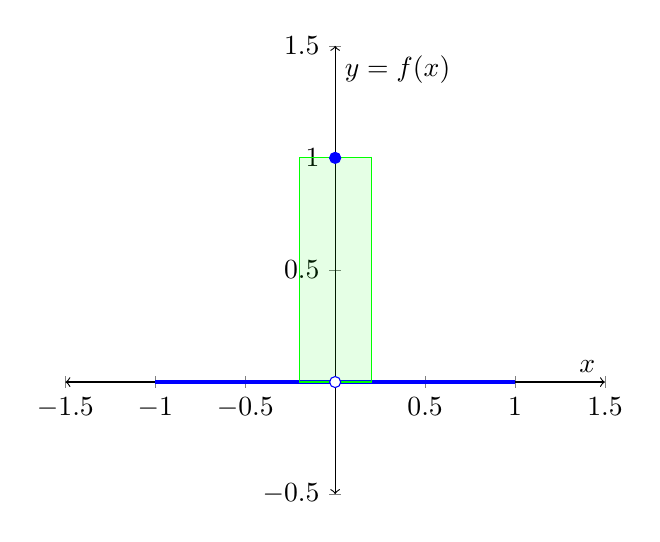
\begin{tikzpicture}
        \begin{axis}[
                xmin=-1.5,xmax=1.5,
                ymin=-0.5,ymax=1.5,
                axis x line=middle,
                axis y line=middle,
                axis line style=<->,
                xlabel={$x$},
                ylabel={$y=f(x)$},
            ]
            \addplot[blue, very thick, domain=-1:1]{0};
            \addplot[blue, soldot] coordinates{(0,1)};
            \addplot[blue, holdot] coordinates{(0,0)};
            \draw[green, fill=green, fill opacity=0.1] (-0.2,0) rectangle (0.2,1);
        \end{axis}
    \end{tikzpicture}
\end{center}
The above diagram depicts the upper sum $L_P(f)$ for some partition $P$, in which the subinterval containing $x=0$ is represented using a green rectangle of arbitrary width. Because this subinterval contains $x=0$, for which $f(x)=1$, its height is this supremal value of 1. All other subintervals, therefore, have a height of zero, and are not included in this diagram. For this partition $P$, we have that the upper sum is simply the area of this rectangle
$$
    U_P(f)=(\text{area of the green rectangle})=1\cdot(\text{width})
$$
Depending on the chosen partition $P$, the width of the green rectangle can be as large or as small as desired; it can be as large as 2, the size of the domain of our integral, or arbitrarily small, but not zero. In other words, the set of all upper sums is simply the set of all areas for some width $0<w\leq 2$.
$$
    \{\text{upper sums}\}=\{1\cdot w:w\in(0,2]\}=(0,2]
$$
Furthermore, the \textit{upper integral}, the infimum of the set of all upper sums is
$$
    \overline{\int_{-1}^{1}}(f)=\inf\{\text{upper sums}\}=\inf(0,2]=0
$$
Therefore, we have that
$$
    \underline{\int_{-1}^{1}}(f)=\overline{\int_{-1}^{1}}(f)=0
$$
and that $f$ is integrable on $[-1,1]$, and $\displaystyle\int_{-1}^1 f(x)dx=0$.
\subsubsection{A Non-Integrable Function}
There are many non-integrable functions, one of the most well known of which is called the Dirichlet function.
$$
    f(x)=\begin{cases}1&\text{if $x\in\Q$}\\0&\text{if $x\notin\Q$}\end{cases}
$$
In other words, $f(x)$ is $1$ if $x$ is a rational number, otherwise, $f(x)=0$. Let us consider the integral of this function on the interval $[0,1]$. To see why this function is not integrable, consider the following theorem.
\begin{theorem}[``Rational Number Theorem'']
    On every interval $[a,b]$ (where $a,b\in\R$ and $a<b$),
    \begin{itemize}
        \item There exists some $x\in[a,b]$ such that $x$ is a rational number ($x\in \Q$)
        \item There exists some $x\in[a,b]$ such that $x$ is an irrational number ($x\notin \Q$)
    \end{itemize}
    In other words, every interval $[a,b]$ contains both rational and irrational numbers.
\end{theorem}
A simple proof for this theorem can be found in the Appendix.\emptyline
Let $P=\{x_0,x_1,x_2,\dots,x_n\}$ be \textit{any} partition of $[0,1]$. For every subinterval $I=[x_{i-1},x_i]$, we have
\begin{itemize}
    \item $m_i=\displaystyle\inf_{x\in[x_{i-1},x_i]}f(x)=0$
    \item $M_i=\displaystyle\sup_{x\in[x_{i-1},x_i]}f(x)=1$
\end{itemize}
The reason for this is that every interval will have both rational and irrational numbers. Therefore, picking any subinterval and evaluating it on the function $f$ will yield a set $S$ for which at least one element is 0 and at least element is 1. Therefore, $\sup S=1$ and $\inf S=0$. As a result, our upper sum (again, for any partition $P$), will consist of only rectangles with height $M_i=1$, the widths of which add up to 1. Thus, we have
$$
    U_P(f)=1\cdot 1=1
$$
Similarly, we also have
$$
    L_P(f)=1\cdot 0=0
$$
Finally, we have
$$
    \overline{\int_{0}^{1}}(f)=\inf\{1\}=1
$$
and
$$
    \underline{\int_{0}^{1}}(f)=\sup\{0\}=0
$$
As we can see, the upper and lower sums are not equal, and thus, $f(x)$ is not integrable on the domain $[0,1]$. It is worth noting that the Dirichlet function \textit{is} integrable using the Lebesgue definition of integral; however, that is outside the scope of this course.
\subsection{Integrals as Limits}
\subsubsection{Introduction}
As stated before in the previous section regarding, \textit{finer} partitions produce lower upper sums and higher lower sums. Because the upper integral is the infimum of all possible upper sums, in a sense, the upper integral is the upper sum for ``the finest'' partition. Similarly, the lower integral is the lower sum for ``the finest'' partition. From this, it follows that if we were to have a limit as ``fineness approaches infinity'', we would be able to define integrals using limits.
\subsubsection{Definitions}
Recall the definition of \textit{fine} partitions.
\begin{definition}[Fine Partitions]
    Let $P$ and $Q$ be partitions of the interval $[a,b]$. \\
    We say $Q$ is \textbf{finer than} $P$ when $P\subseteq Q$.
\end{definition}
\begin{definition}[Norm of a Partition]
    Let $P=\{x_0,x_1,x_2,\dots,x_n\}$ be a partition of $[a,b]$. \\
    For each $i=1,2,\dots, n$, let $\Delta x_i=x_i-x_{i-1}$. \\
    The \textbf{norm} of $P$ is
    $$
        \norm{P}=\max\{\Delta x_1,\Delta x_2,\dots,\Delta x_n\}
    $$
\end{definition}
\subsubsection{Integrals as Limits}
From the above two definitions, we have the following theorem:
\begin{theorem}
    Let $f$ be a bounded function on $[a,b]$.
    $$
        \underline{\int_a^b}(f)=\lim_{\norm{P}\to 0} L_P(f)
    $$
    and
    $$
        \overline{\int_a^b}(f)=\lim_{\norm{P}\to 0} U_P(f)
    $$
\end{theorem}
What this theorem states is that
$$
    \forall \varepsilon>0,~\exists \delta>0~~\text{such that}~~\forall\text{partition $P$ of $[a,b]$},~\norm{P}<\delta\implies \left|\underline{\int_a^b}(f)-L_P(f)\right|<\varepsilon
$$
and
$$
    \forall \varepsilon>0,~\exists \delta>0~~\text{such that}~~\forall\text{partition $P$ of $[a,b]$},~\norm{P}<\delta\implies \left|\overline{\int_a^b}(f)-U_P(f)\right|<\varepsilon
$$
In other words, as the norm of a partition $P$ approaches zero, the difference between its lower sum and the actual lower integral also approaches zero. The same is true for upper sums.
\emptyline
Because this theorem involves the domain of all possible partitions for a given interval $[a,b]$, it does not simplify computation. By defining a specific way in which the norm of our partitions approaches zero, we can simplify this definition.
\begin{theorem}
    Pick a sequence of partitions $P_1,P_2,P_3,\dots$ for the interval $[a,b]$ satisfying
    $$
        \lim_{n\to\infty}\norm{P_n}=0
    $$
    Then,
    $$
        \underline{\int_a^b}(f)=\lim_{n\to\infty}L_{P_n}(f)
    $$
    and
    $$
        \overline{\int_a^b}(f)=\lim_{n\to\infty}U_{P_n}(f)
    $$
    \hr
    The simplest example of such a sequence is the sequence that breaks the interval $[a,b]$ into $n$ equally sized subintervals:
    $$
        P_n=\left\{a+\frac{t(b-a)}{n}:t\in\{0,1,2,\dots,n\}\right\}
    $$
\end{theorem}
This definition of integral using limits is more useful than the previous one, since it takes the more intuitive concept of some number approaching infinity, rather than the norm of a partition approaching zero across the domain of all partitions.
\subsubsection{The ``$\varepsilon$-Characterization'' of Integrability}
\begin{theorem}
    Let $f$ be a bounded function on $[a,b]$. \\
    IF $f$ is integrable on $[a,b]$,
    THEN
    $$
        \forall \varepsilon>0,~\exists~\text{a partition $P$ of $[a,b]$}~~\text{such that}~~U_P(f)-L_P(f)<\varepsilon
    $$
\end{theorem}
The above theorem represents a way to show that integrable functions can be characterized using a definition similar to that of a limit. One way to prove this theorem is by using the delta-epsilon definition of limit to construct an interval on which $f(x)$ is strictly positive. From there, we can prove that there exists at least one non-zero lower sum. By the properties of lower and upper sums then, all upper sums are also non-zero.
\newpage
\begin{proof}
    From the definition of integral as a limit, we have
$$
    \lim_{n\to\infty} L_{P_n}(f)=\underline{\int_a^b}(f)
    \quad\text{and}\quad
    \lim_{n\to\infty} U_{P_n}(f)=\overline{\int_a^b}(f)
$$
For a sequence of partitions $P_1,P_2,P_3,\dots$ for the interval $[a,b]$ for which $\displaystyle\lim_{n\to\infty}\norm{P_n}=0$.
From the limit definition, then, we have 
$$
    \forall \varepsilon>0,~\exists M>0\suchthat n>M\implies \underline{\int_a^b}(f)-L_{P_n}(f)<\varepsilon
$$
Because the lower integral is always greater than or equal to all lower sums, we can order the terms as such without need for taking an absolute value. From this statement, we more loosely say that
$$
    \forall \varepsilon>0,~\exists \text{partition $P_1$}\suchthat\underline{\int_a^b}(f)-L_{P_1}(f)<\varepsilon
$$
By a similar reasoning for upper sums, we have that
$$
    \forall \varepsilon>0,~\exists \text{partition $P_2$}\suchthat U_{P_2}(f)-\overline{\int_a^b}(f)<\varepsilon
$$
Because we also have that $f$ is integrable on $[a,b]$, then we have that the lower and upper integrals are equal. Thus, let $I=\int_a^bf(x)dx = \underline{\int_a^b}(f) = \overline{\int_a^b}(f)$. Combining this fact with the above two statements, we get that
$$
    \forall \varepsilon>0,~\exists \text{partitions $P_1,P_2$}\suchthat I-L_{P_1}<\varepsilon\text{~~and~~}U_{P_2}-I<\varepsilon
$$
Because we also know that $L_{P_1}\leq I \leq U_{P_2}$, we have that
$$
    I-\varepsilon < L_{P_1} \leq I \leq U_{P_2} < I+\varepsilon
$$
Here is a diagram of this inequality:
\begin{center}
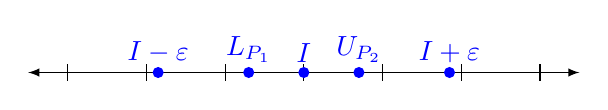
\begin{tikzpicture}
\draw[latex-latex] (-3.5,0) -- (3.5,0) ; %edit here for the axis
\foreach \x in  {-3,-2,-1,0,1,2,3} % edit here for the vertical lines
\draw[shift={(\x,0)},color=black] (0pt,3pt) -- (0pt,-3pt);
\fill[blue] (0,0) circle (0.2em) node[anchor=south]{$I$};
\fill[blue] (0.7,0) circle (0.2em) node[anchor=south]{$U_{P_2}$};
\fill[blue] (-0.7,0) circle (0.2em) node[anchor=south]{$L_{P_1}$};
\fill[blue] (1.85,0) circle (0.2em) node[anchor=south]{$I+\varepsilon$};
\fill[blue] (-1.85,0) circle (0.2em) node[anchor=south]{$I-\varepsilon$};
\end{tikzpicture}
\end{center}
The distance between $I+\varepsilon$ and $I-\varepsilon$ is $2\varepsilon$. Because $L_{P_1}$ and $U_{P_2}$ are bounded by these two endpoints, their distance cannot exceed $2\varepsilon$. Thus, we have
$$
    U_{P_2}-L_{P_2}<2\varepsilon
$$
Let $P_3=P_1\cup P_2$. Because $P_2\subseteq P_3$ and $P_1\subseteq P_3$, we say that $P_3$ is \textit{finer} than both $P_1$ and $P_2$, and we have the inequality
$$
    L_{P_1}\leq L_{P_3} \leq I \leq U_{P_3} \leq U_{P_2}
$$
As $L_{P_3},U_{P_3}$ are bounded by $L_{P_1}$ and $U_{P_2}$ respectively, we have also that $U_{P_3}-L_{P_3}<2\varepsilon$. Having shown that the original statement is true for twice the value of any arbitrary value of $\varepsilon>0$, we have also shown this to be true for all $\varepsilon$.
\end{proof}
\subsection{Riemann Sums \& Riemann Integration}
\subsubsection{Definition}
\begin{definition}
    Let $f$ be a bounded function on the interval $[a,b]$. \\
    Let $P=\{x_0,x_1,x_2,\dots,x_n\}$ be a partition of $[a,b]$. \\
    For each $i=1,2,\dots,n$:
    \begin{itemize}
        \item Let $\Delta x_i=x_i-x_{i-1}$
        \item Choose a number $x_i^*\in[x_{i-1},x_i]$ (for simplicity, we can take $x_i^*=x_{i-1}$ or $x_i^*=x_i$)
    \end{itemize}
    Then
    $$
        S_P^*(f)=\sum_{i=1}^nf(x_i^*)\cdot\Delta x_i
    $$
    is called a \textbf{Riemann sum} for $f$ and $P$.
\end{definition}
Notice that we say \textit{a} Riemann sum rather than \textit{the} Riemann sum. Because we arbitrarily choose $x_i^*$, there are infinitely many Riemann sums. One common choice is to take $x_i^*=x_{i-1}$. This is called a \textit{left Riemann sum}, because it uses the left-hand value of each subinterval. To denote this choice of $x_i^*$, we denote the Riemann sum $S_P^*$.
\subsubsection{Riemann Integrals}
The relationship between Riemann sums and integrals can be summarized in the following theorem:
\begin{theorem}[``Riemann Integral Theorem'']
    Let $f$ be a bounded function on the interval $[a,b]$. Assume $f$ is integrable on $[a,b]$.
    \begin{itemize}
        \item Pick a sequence of partitions $P_1,P_2,P_3,\dots$ for the interval $[a,b]$ satisfying
        $$
            \lim_{n\to\infty}\norm{P_n}=0
        $$
        \item On each subinterval of each partition, pick $x_i^*\in[x_{i-1},x_i]$.
    \end{itemize}
    Then
    $$
        \int_a^b f(x)dx=\lim_{n\to\infty} S_{P_n}^*(f)
    $$
    \hr
    \begin{itemize}
        \item The simplest example of such a sequence is the sequence that breaks the interval $[a,b]$ into $n$ equally sized subintervals:
        $$
            P_n=\left\{a+\frac{t(b-a)}{n}:t\in\{0,1,2,\dots,n\}\right\}
        $$
        \item The simplest choice of $x_i^*$ would be $x_i^*=x_i$
    \end{itemize}
\end{theorem}
\textit{(A proof for the above theorem is included in the Appendix)} \emptyline
Sometimes, this theorem is represented using the single formula:
$$
    \textcolor{blue}{\int_a^b} f(x)\textcolor{red}{dx}=\lim_{n\to\infty}\left[\textcolor{blue}{\sum_{i=1}^n} f(x_i^*)\cdot\textcolor{red}{\Delta x_i}\right]\footnote{Strictly speaking, $x_i^*$ and $x_i$ should also depend on $n$, but this is standard notation.}
$$
In a sense, the integral and the sum, labeled in blue represent the same concept, as does $dx$ compared to $\Delta x_i$ in red.
\subsubsection{Computing Definite Integrals using Riemann Sums - Example 1}
Calculate
$$
    \int_0^1 f(x) dx\quad\text{where $f(x)=x$}
$$
using Riemann sums.
It should be immediately apparent, without any calculations, that the integral is one-half.
\begin{center}
    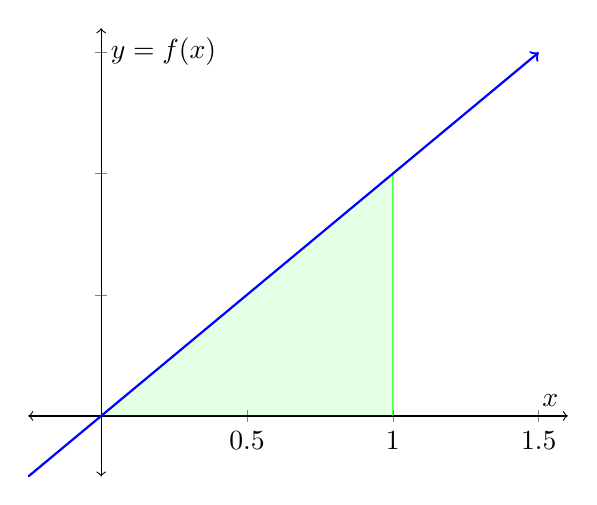
\begin{tikzpicture}
        \begin{axis}[
                xmin=-0.25,xmax=1.6,
                ymin=-0.25,ymax=1.6,
                axis x line=middle,
                axis y line=middle,
                axis line style=<->,
                xlabel={$x$},
                ylabel={$y=f(x)$},
                yticklabels=\empty
            ]
            \draw[green, fill=green, fill opacity=0.1] (0,0) -- (1,1) -- (1,0);
            \addplot[blue, thick, domain=-1:1.5, ->]{x};
        \end{axis}
    \end{tikzpicture}
\end{center}
Therefore, if the answer reached is also one-half, we know it is correct. Let us begin by choosing $P_n$ by breaking $[0,1]$ into $n$ equal subintervals:
$$
    P_n=\left\{\frac{t}{n}:t\in\{0,1,2,\dots,n\}\right\}=\left\{0,\frac{1}{n},\frac{2}{n},\frac{3}{n},\dots,1\right\}
$$
Let us also define $x_i^*$ to be the right endpoint of every subinterval. If we have $x_i^*$ corresponding to the subinterval $[x_{i-1},x_i]$, then the right endpoint is $x_i$. Since we have
$$
    P_n=\{x_0,x_1,x_2,\dots,x_n\}=\left\{0,\frac{1}{n},\frac{2}{n},\frac{3}{n},\dots,1\right\}
$$
notice that each element of $P$, denoted $x_i$, corresponds to the element $\frac{i}{n}$. Therefore, for every subinterval, we have
$$
    x_i^*=\frac{i}{n}
$$
Remember that a Riemann sum is calculated as
$$
    S_P^*(f)=\sum_{i=1}^nf(x_i^*)\cdot\Delta x_i
$$
Each interval is evenly spaced. Subinterval $x_i$ corresponds to $\frac{i}{n}$, so we have the width of any subinterval, $\Delta x_i$ computed as
$$
    \Delta x_i=x_{i+1}-x_i=\frac{i+1}{n}-\frac{i}{n}=\frac{1}{n}
$$
Again, we defined $x_i^*$ to be $\frac{i}{n}$, so substituting values of $x_i^*$ and $\Delta x_i$ gives us
$$
    S_P^*(f)=\sum_{i=1}^nf\left(\frac{i}{n}\right)\cdot\frac{1}{n}
$$
Since we have $f(x)=x$, we have
$$
    S_P^*(f)=\sum_{i=1}^n\frac{i}{n}\cdot\frac{1}{n}
$$
Then, to compute the integral from the Riemann sums, we have
$$
    \begin{aligned}
        \int_0^1 f(x) dx&=\lim_{n\to\infty}\left[\sum_{i=1}^n\frac{i}{n}\cdot\frac{1}{n}\right] \\
        &=\lim_{n\to\infty}\left[\sum_{i=1}^n i\cdot \frac{1}{n^2}\right]
    \end{aligned}
$$
Because $\frac{1}{n^2}$ is a constant in the context of {\footnotesize$\displaystyle\lim_{n\to\infty}$}, we then have
$$
    \begin{aligned}
        \lim_{n\to\infty}\left[\sum_{i=1}^n i\cdot \frac{1}{n^2}\right] &= \lim_{n\to\infty}\left[\frac{1}{n^2}\sum_{i=1}^n i\cdot\right] \\
        &=\lim_{n\to\infty}\left[\frac{1}{n^2}\cdot\frac{n(n+1)}{2}\right] \\
        &=\lim_{n\to\infty}\left[\frac{n(n+1)}{2n^2}\right] \\
        &=\lim_{n\to\infty}\left[\frac{n+1}{2n}\right] \\
        &=\frac{1}{2}
    \end{aligned}
$$
Finally, we have
$$
    \int_0^1f(x)dx=\frac{1}{2}
$$
\subsubsection{Computing Definite Integrals using Riemann Sums - Example 2}
Let $f(x)=x^2-x+1$. Compute
$$
    \int_0^2 f(x)dx
$$
Following a similar process as before, let us define our sequence of partitions $P_n$ to divide $[0,2]$ into $n$ equally-sized subintervals as so:
$$
    P_n=\left\{\frac{2t}{n}:t\in\{0,1,2,\dots,n\}\right\}=\left\{\frac{0}{n},\frac{2}{n},\frac{4}{n},\dots,\frac{2n}{n}\right\}
$$
let $x_i^*$ be the right endpoint,
$$x_i^*=x_i=\frac{2i}{n}$$
and let
$$
    \Delta x_i=x_{i+1}-x_i=\frac{2(i+1)}{n}-\frac{2i}{n}=\frac{2i+2-2i}{n}=\frac{2}{n}
$$
Then we have
$$
   \begin{aligned}
        S_P^*(f)&=\sum_{i=1}^n f(x_i^*)\cdot\Delta x_i \\
        &=\sum_{i=1}^n f\left(\frac{2i}{n}\right)\cdot\frac{2}{n} \\
        &=\sum_{i=1}^n\left(\frac{4i^2}{n^2}-\frac{2i}{n}+1\right)\left(\frac{2}{n}\right) \\
        &=\sum_{i=1}^n\left(\frac{8i^2}{n^3}-\frac{4i}{n^2}+\frac{2}{n}\right) \\
        &=\sum_{i=1}^n\left(\frac{8i^2}{n^3}\right)-\sum_{i=1}^n\left(\frac{4i}{n^2}\right)+\sum_{i=1}^n\left(\frac{2}{n}\right)
   \end{aligned}
$$
Then we have 
$$
    \begin{aligned}
         \int_0^2f(x)dx=\lim_{n\to\infty}\left[S_{P_n}^*(f)\right]&=\lim_{n\to\infty}\left[\sum_{i=1}^n\left(\frac{8i^2}{n^3}\right)-\sum_{i=1}^n\left(\frac{4i}{n^2}\right)+\sum_{i=1}^n\left(\frac{2}{n}\right)\right] \\
         &=\lim_{n\to\infty}\left[
            \left(\frac{8}{n^3}\sum_{i=1}^ni^2\right) - 
            \left(\frac{4}{n^2}\sum_{i=1}^ni\right) +
            \left(\frac{2}{n}\sum_{i=1}^n1\right)
        \right] \\
        &=\lim_{n\to\infty}\left[
            \left(\frac{8}{n^3}\cdot\frac{n(n+1)(2n+1)}{6}\right) -
            \left(\frac{4}{n^2}\cdot\frac{n(n+1)}{2}\right) +
            \left(\frac{2}{n}\cdot n\right)
        \right] \\
        &=\lim_{n\to\infty}\left[\frac{8(n+1)(2n+1)}{6n^2}\right]-\lim_{n\to\infty}\left[\frac{4(n+1)}{2n}\right]+2 \\
        &=\frac{16}{6}-2+2 \\ 
        &=\frac{8}{3}\approx2.667
    \end{aligned}
$$
\newpage
\subsection{Properties of Definite Integrals}
\subsubsection{Arithemetic Properties}
Definite integrals follow similar properties to sums ($\Sigma$). Assuming $f$ and $g$ are integrable on $[a,b]$, we have
$$
    \int_a^b\big[f(x)+g(x)\big]dx=\int_a^bf(x)dx+\int_a^bg(x)dx
$$
and
$$
    \int_a^b\big[cf(x)\big]dx=c\cdot\int_a^bf(x)dx
$$
where $c$ is some constant.
\subsubsection{Definite Integrals over Different Intervals}
Let $f$ be some function integrable on $[a,b]$ and on $[b,c]$.
\begin{center}
    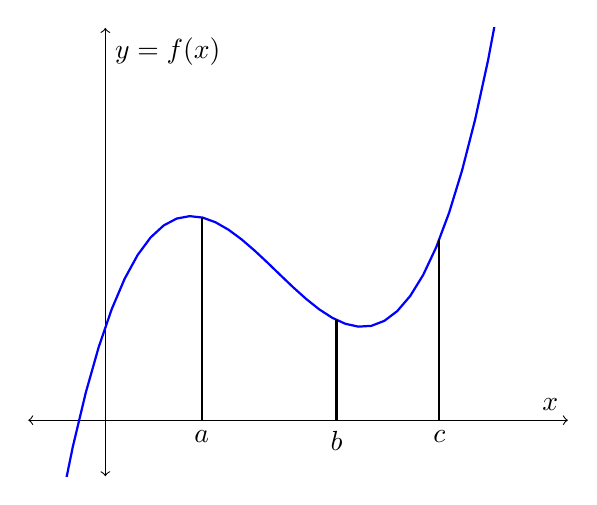
\begin{tikzpicture}
        \begin{axis}[
                xmin=-0.6,xmax=3.6,
                ymin=-0.6,ymax=4.2,
                axis x line=middle,
                axis y line=middle,
                axis line style=<->,
                xlabel={$x$},
                ylabel={$y=f(x)$},
                xtick=\empty,
                ytick=\empty
            ]
            \addplot[blue, thick, samples=100, name path=f]{x*x*x-4*x*x+4*x+1};
            \draw[black, thick] (0.75,0) node[anchor=north]{$a$} -- (0.75,2.17);
            \draw[black, thick] (1.8,0) node[anchor=north]{$b$} -- (1.8,1.072);
            \draw[black, thick] (2.6,0) node[anchor=north]{$c$} -- (2.6,1.936);
        \end{axis}
    \end{tikzpicture}
\end{center}
$$
    \int_a^cf(x)dx=\int_a^bf(x)dx+\int_b^cf(x)dx
$$
Note that this property is true, regardless of the order of $a$, $b$, and $c$.
\subsubsection{Backwards and Zero Integrals}
Reversing the bounds of a definite integral reverses the sign of its value.
$$
    \int_b^a f(x)dx = -\int_a^b f(x)dx
$$
A definite integral over a zero-width interval is zero, even if the function is not integrable.
$$
    \int_a^a f(x)dx=0
$$
\subsubsection{Integrals of Smaller Functions}
If for all values of $x$ on the interval $[a,b]$, we have that $f(x)\leq g(x)$, then
$$
    \int_a^b f(x)dx \leq \int_a^b g(x)dx
$$
\section{Unit 8: The Fundamental Theorem of Calculus}
\subsection{Antiderivatives and Indefinite Integrals}
\subsubsection{Introduction}
So far, we have only been dealing with definite integrals, expressions of the form
$$
    \int_a^bf(x)dx
$$
The value of this expression is a single number. Geometrically, it measures the ``area under the curve'', more specifically, the area of the function above the $x$-axis minus the area below the $x$-axis. This unit will focus on the notion of indefinite integrals, written the same way, but without the notion of ``from $a$ to $b$'':
$$
    \int f(x)dx
$$
\subsubsection{Definitions}
\begin{definition}
    Let $f$ be a function defined on an interval.
    \begin{itemize}
        \item An \textbf{antiderivative} of $f$ is any function $F$ such that $F'=f$
        \item The collection of all antiderivatives of $f$ is denoted $\displaystyle\int f(x)dx$
    \end{itemize}
\end{definition}
As an example, consider $\displaystyle \int f(x)dx$ where $f(x)=x^2$. Intuitively, by reversing the process involved in the power rule, we see that $F(x)=\frac{1}{3}x^3$ is one antiderivative for $f$. We can verify that this is correct by taking its derivative.
$$
    \frac{d}{dx}\left[\frac{1}{3}x^3\right]=x^2
$$
However, because the derivative of any constant is zero, we can also add any constant $C$ to $F$. In other words,
$$
    \forall C\in\R,~\frac{d}{dx}F(x)=f(x)\quad\text{where}~F(x)=\frac{1}{3}x^3+C
$$
\subsubsection{Examples - Initial Value}
Consider a function $f$ such that $f'(x)=2x+1$. Such a function would follow the form
$$
    f(x)=x^2+x+C
$$
Say we are given that $f(0)=1$. Then, we can find an exact value for our constant $C$.
$$
    f(x)=x^2+c+1
$$
In general, for any functions $f(x)$ and $g(x)$ such that $f'(x)=g(x)$, we will have
$$
    f(x)=\dots+C
$$
If we have $C=0$, $f(0)$ will always equal zero. Therefore, if we are given a fixed value $a=f(0)$, then we have explicitly that
$$
    f(x)=\dots+a
$$
If we are given a point on $f$ where $x\neq 0$, we can still determine an explicit expression for $f$. Imagine we are given $f'(x)=2x+1$ and $f(2)=8$. We know that
$$
    f(x)=x^2+x+C
$$
To resolve an explicit expression for $f$, we can simply solve for $C$. Knowing that $f(2)=8$, we can substitute $x$ for $\textcolor{red}{2}$ and $f(x)$ for $\textcolor{blue}{8}$ to get the equation
$$
    \textcolor{blue}{8}=(\textcolor{red}{2})^2+(\textcolor{red}{2})+C
$$
Solving this equation gives us $C=2$. Therefore, we have
$$
    f(x)=x^2+x+2
$$
\subsubsection{Examples - Antiderivatives of Graphed Functions}
Here is an example of a common question asked in calculus classes. \\
\textbf{Given the graph of the function $f'(x)$ below, sketch a graph of $f(x)$ where $f(0)=0$}. 
\begin{center}
    \begin{tikzpicture}
        \begin{axis}[
                xmin=-1.4,xmax=3.6,
                ymin=-1.2,ymax=2.6,
                axis x line=middle,
                axis y line=middle,
                axis line style=<->,
                xlabel={$x$},
                ylabel={$y=\frac{d}{dx}f(x)$},
            ]
            \addplot[blue, thick, samples=100, domain=-2:1]{x};
            \addplot[blue, thick, samples=100, domain=1:2]{1};
            \addplot[blue, thick, samples=100, domain=2:4]{-x+3};
        \end{axis}
    \end{tikzpicture}
\end{center}
As an analogy, consider the graph of $f'(x)$ to be a graph of the velocity of a car with respect to time. The graph of $f(x)$, then, its a graph of its position. From $x\in[-1,1]$, we have that the car is moving in the negative direction, but it is accelerating in the positive direction. At $x=0$, it briefly comes to a complete stop, and its position is zero. But then, it keeps accelerating until $x=1$, at which point, it maintains its current velocity until $x=2$, at which point it begins to slow down, eventually moving again in the negative direction.\emptyline
Here is the ``answer'' to this question:
\begin{center}
    \begin{tikzpicture}
        \begin{axis}[
                xmin=-1.4,xmax=3.6,
                ymin=-1.2,ymax=2.6,
                axis x line=middle,
                axis y line=middle,
                axis line style=<->,
                xlabel={$x$},
                ylabel={$y=\frac{d}{dx}f(x)$},
            ]
            \addplot[blue, thick, samples=100, domain=-2:1]{0.5*x^2};
            \addplot[blue, thick, samples=100, domain=1:2]{x-0.5};
            \addplot[blue, thick, samples=100, domain=2:4]{-0.5*(x-3)^2+2};
        \end{axis}
    \end{tikzpicture}
\end{center}
Notice the straight line (``constant velocity'') segment from $x=1$ to $x=2$ and the ``acceleration'' elsewhere. Notice also, that when the graph of $f'(x)$ touches zero, the graph of $f(x)$ ``stops moving'' briefly ($f$ has a critical point).
\emptyline
Another way to look at these types of problems is by evaluating the type of curvature of $f'(x)$ along segment. For instance, from $x\in[-1,1]$, we have that the graph of $f'(x)$ is linear. Intuitively, then, we know that its antiderivative along that interval should be a quadratic. Similarly, constant segments of $f'(x)$ should correspond to linear antiderivatives, and quadratic or parabolic-seeming segments of $f'(x)$ should roughly correspond to cubic antiderivatives.
\subsubsection{Functions Defined as Integrals}
Recall the earlier definition of antiderivative.
\begin{definition}
    Let $f$ be a function defined on an interval.
    \begin{itemize}
        \item An \textbf{antiderivative} of $f$ is any function $F$ such that $F'=f$
        \item The collection of all antiderivatives of $f$ is denoted $\displaystyle\int f(x)dx$
    \end{itemize}
\end{definition}
We can define $F$ using a definite integral. If we use an earlier analogy that $\displaystyle\int_a^bf(x)dx$ ``tracks'' the position of a car from $a$ to $b$ with a velocity given as $f(x)$ and returns the position of the car at $b$, we can define a function that tracks the value at any arbitrary point by using its argument as the endpoint of the integral.
\emptyline
Let $I$ be an interval. \\
Let $a\in I$. \\
Let $f$ b ea function integrable on $I$. \\
Then,
$$
    \forall x\in I,~F(x)=\int_a^x f(t)dt~~~~\text{is a valid way to define $F$}
$$
Note that we say $f(t)dt$ instead of $f(x)dx$ since $x$ is already being used. Remember that the choice of integration variable is irrelevant. By convention, we often use $t$. Also note that the choice of $a$ does not inherently change the ``shape'' of $F$, it only moves it up or down.
\subsection{The First Fundamental Theorem of Calculus}
\subsubsection{Introduction}
The fundamental theorem of calculus (FTC) is a theorem that relates the derivative of a function to its integral. In other words, it is a theorem that shows that integration is essentially an inverse operation to differentiation, and vice versa. The fundamental theorem of calculus has two parts; the first part defines the concept of an antiderivative, and the second defines a way to compute definite integrals.
\subsubsection{Definitions}
\begin{theorem}[Fundamental Theorem of Calculus - Part 1]
    Let $[a,b]$ be a closed interval. \\
    Let $f$ be a continuous (and therefore integrable) function on $[a,b]$. \\
    We define
    $$
        F(x)=\int_a^xf(t)dt
    $$
    Then $f$ is differentiable on the open interval $(a,b)$ and $F'=f$, that is,
    $$
        \forall x\in (a,b),~F'(x)=f(x)
    $$
\end{theorem}\footnote{The MAT137 Video 8.3 defines the FTC Part 1 differently. The one written above should be more technically accurate.}
A common way to summarize the above theorem is the statement that ``a function defined as an integral is an antiderivative''.
$$
    \frac{d}{dx}\int_a^x f(t)dt=f(x)
$$
\subsubsection{Example 1}
Let
$$
    F(x)=\int_1^x e^{-t^2}dt
$$
What is $F'(2)$?
\begin{solution}
    Notice that
    $$
        \frac{d}{dx}F(x)=\frac{d}{dx}\int_a^xe^{-t^2}dt=e^{-x^2}
    $$
    Therefore, $F(x)=e^{-(-2)^2}=e^{-4}$.
\end{solution}
\subsubsection{Example 2}
Construct a function $g$ such that for all $x\in\R$,
$$
    g'(x)=\frac{1}{1+x^2+x^{10}}
$$
and $g(2)=5$.
\begin{solution}
    By the first fundamental theorem of calculus, we have that the antiderivative of $g'(x)$ can be written as an integral. Remember also, that for any antiderivative $f(x)$ defined in this way, $f(x)=\displaystyle\int_a^x\dots$, we have that $f(a)=0$. Therefore, we have
    $$
        g(x)=5+\int_2^x\frac{1}{1+t^2+t^{10}}dt
    $$
\end{solution}
\newpage
\subsubsection{Example 3}
Let
$$
    G(x)=\int_{-4}^{x^2} \frac{\sin t}{t}dt
$$
Calculate $G'(x)$.
\begin{solution}
    First, let us define
    $$
        F(x)=\int_{-4}^x\frac{\sin t}{t} dt
    $$
    By the first fundamental theorem of calculus, we have
    $$
        F'(x)=\frac{d}{dx}\int_{-4}^x\frac{\sin t}{t}dt=\frac{\sin x}{x}
    $$
    We also know that
    $$
        G(x)=F(x^2)
    $$
    Then,
    $$
        G'(x)=\frac{d}{dx}F(x^2)=2xF'(x^2)=\frac{2x\sin x^2}{x^2}
    $$
\end{solution}
\subsubsection{Example 4}
Let
$$
    H(x)=\int_{x^3+1}^{x^2+2x} e^{-t^2}dt
$$
Calculate $H'(x)$.
\begin{solution}
    Recall an earlier property of definite integrals:
    $$
        \int_a^cf(x)dx=\int_a^bf(x)dx+\int_b^cf(x)dx
    $$
    This property is true, regardless of the order of $a$, $b$, and $c$. So, we have
    $$
        H(x)=\int_{x^3+1}^{x^2+2x} e^{-t^2}dt = \int_{x^3+1}^0 e^{-t^2}d+ \int_0^{x^2+2x}e^{-t^2}d
    $$
    Then, let
    $$
        F(x)=\int_x^{0} e^{-t^2}dt\quad\text{and}\quad G(x)=\int_{0}^x e^{-t^2}d
    $$
    We have
    $$
        H(x)=F(x^3+1)+G(x^2+2x)
    $$
    Then,
    $$
        \begin{aligned}
             H'(x) &=3 x^2F'(x^3+1)+(2x+2)G'(x^2+2x)
        \end{aligned}
    $$
    By the first fundamental theorem of calculus, we can create explicit expressions for $F'(x)$ and $G'(x)$
    $$
        \begin{aligned}
            &F'(x)=\frac{d}{dx}\int_x^0 e^{-t^2}dt=\frac{d}{dx}\left(-\int_0^xe^{-t^2}\right)=-e^{-x^2} \\
            &G'(x)=\frac{d}{dx}\int_0^xe^{-t^2}dt=e^{-x^2}
        \end{aligned}
    $$
    From there, we have
    $$
        H'(x)=3x^2\cdot\left(-e^{-(x^3+1)^2}\right)+(2x+2)\left(e^{-(x^2+2x)^2}\right)
    $$
\end{solution}
The processes used in examples 3 and 4 can be summarized using the following formula.
\subsubsection{Generalized Version of the First Fundamental Theorem of Calculus}
Let $f,u,v$ be differentiable functions with domain $\R$. Let
$$
    F(x)=\int_{u(x)}^{v(x)}f(t)dt
$$
Given that we can write $F(x)$ as 
$$
    F(x)=\int_{u(x)}^0f(t)dt+\int_{0}^{v(x)}f(t)dt
$$
We have
$$
    F'(x)=-f(u(x))\cdot u'(x)+f(v(x))\cdot v'(x)
$$
\newpage
\subsection{The Second Fundamental Theorem of Calculus}
\subsubsection{Definition}
\begin{theorem}
Let $a<b$. \\
Let $f$ be continuous on $[a,b]$. \\
Let $F$ be any antiderivative of $f$. ($F'(x)=f(x)$) \\
Then,
$$
    \int_a^b f(x)dx=F(b)-F(a)  
$$
\end{theorem}
Because the value represented by the expression $F(b)-F(a)$ is used very commonly, we often write $\displaystyle F(x)\Big|_a^b$, pronounced ``$F(x)$ evaluated from $a$ to $b$''. In summary, we have
$$
    \int_a^bf(x)dx=F(x)\Big|_a^b=F(b)-F(a)
$$
\subsubsection{Example}
Compute
$$
    \int_1^2x^2dx
$$
\begin{solution}
    First, we need to find an antiderivative of $x^2$. Intuitively, we have $\frac{1}{3}x^3$ as one such antiderivative. Therefore, we have
    $$
        \int_1^2x^2dx=\frac{1}{3}x^3\Big|_1^2=\left(\frac{1}{3}(2)^3\right)-\left(\frac{1}{3}(1)^3\right)=\frac{8}{3}-\frac{1}{3}=\frac{7}{3}
    $$
\end{solution}
\subsection{The Three Notions of Integral - A Summary}
\subsubsection{Introduction}
So far, three ways of representing integrals have been presented. \\
We have definite integrals, written
$$
    \int_a^b f(x)dx
$$
We have indefinite integrals, written
$$
    \int f(x)dx
$$
And we have functions defined as integrals, written
$$
    F(x)=\int_a^xf(t)dt
$$
\subsubsection{Definite Integrals}
$$
    \int_a^b f(x)dx
$$

\section{Unit 9: Integration Methods}


%% APPENDIX %%
\section{Appendix}
\subsection{Proof of the ``Rational Number Theorem''}
\begin{proof}
    Let $a,b\in\R$ such that $a<b$. \\
    Consider a natural number $n$ such that
    $$
        \frac{\sqrt 2}{n}<b-a
    $$
    (Such a number can be found by taking $\ceil*{\frac{\sqrt 2}{b-a}}$). \\
    Let $w=\frac{\sqrt{2}}{n}$. Notice that $w$ is an irrational number, since $\sqrt{2}$ is irrational. Additionally, $w+a$ is irrational. We also have $a<a+w<b$, since $w<b-a$. Thus, $w+a\notin\Q$ and $w+a\in[a,b]$. To instead find a \textit{rational} number, take $\frac{1}{n}$ instead of $\frac{\sqrt{2}}{n}$.
\end{proof}
\subsection{Proof of the ``Riemann Integral Theorem''}
\begin{proof}
    We start by assuming the following statements for any bounded function $f$:
    \begin{itemize}
        \item $\displaystyle\lim_{n\to\infty}L_{P_n}(f)=\underline{\int_a^b}(f)$
        \item $\displaystyle\lim_{n\to\infty}U_{P_n}(f)=\overline{\int_a^b}(f)$
    \end{itemize}
    However, from our hypothesis, we have that $f$ is integrable, we also have that the upper and lower integrals are equal. Thus,
    $$
        \lim_{n\to\infty} L_{P_n}(f)=\lim_{n\to\infty} U_{P_n}(f) = \int_a^b f(x)dx
    $$
    Additionally, we have
    $$
        L_{P_n}(f)\leq S_{P_n}^*(f)\leq U_{P_n}(f)
    $$
    Then, from the Squeeze Theorem,
    $$
        \lim_{n\to\infty} S_{P_n}^*(f)=\int_a^bf(x)dx
    $$
\end{proof}
\end{document}
